\documentclass[11pt,a4paper]{article}
\usepackage[utf8]{inputenc}
\usepackage[T1]{fontenc}
\usepackage{amsthm} %numéroter les questions
\usepackage[english]{babel}
\usepackage{datetime}
\usepackage{xspace} % typographie IN
\usepackage{hyperref}% hyperliens
\usepackage[all]{hypcap} %lien pointe en haut des figures

\usepackage{fancyhdr}% en têtes
\usepackage{graphicx} %include pictures
\usepackage{pgfplots}

% \usepackage{minted}
\usepackage{colortbl}
\usepackage{tikz}
\usetikzlibrary{calc}
\usetikzlibrary{babel}
\usetikzlibrary{tikzmark}

\usepackage{circuitikz}
% \usepackage{gnuplottex}
\usepackage{float}
\usepackage{ifthen}

\usepackage[top=1.3 in, bottom=1.3 in, left=1.3 in, right=1.3 in]{geometry}
\usepackage[]{pdfpages}
\usepackage[]{attachfile}

\usepackage{amsmath}
\usepackage{enumitem}
\setlist[enumerate]{label=\alph*)}% If you want only the x-th level to use this format, use '[enumerate,x]'
\usepackage{multirow}

\usepackage{aeguill} %guillemets


%%%%%%%%%%%%%%%%%%%%%%%%%%%%%%%%%%%%%%%%%%%%%%%%%%%%%%%%%%%%%%%%%%%%%%%%%%%%%%%%%%%%%%%%%%%
% READ THIS BEFORE CHANGING ANYTHING
%
%
% - TP number: can be changed using the command
%		\def \tpnumber {TP 1 }
%
% - Version: controlled by a new command:
%		\newcommand{\version}{v1.0.0}
%
% - Booleans: there are three booleans used in this document:
%	- 'corrige', controlled by defining the variable 'corrige'
% You can define those variables in a makefile using such a command:
% pdflatex -shell-escape -jobname="infoh410_tp1" "\def\corrige{} \input{infoh410_tp1.tex}"
%
%%%%%%%%%%%%%%%%%%%%%%%%%%%%%%%%%%%%%%%%%%%%%%%%%%%%%%%%%%%%%%%%%%%%%%%%%%%%%%%%%%%%%%%%%%%

%Numero du TP :
\def \tpnumber {TP RL (Reinforcement learning)}

\newcommand{\version}{v1.0.0}


% ########     #####      #####    ##         #########     ###     ##      ##  
% ##     ##  ##     ##  ##     ##  ##         ##           ## ##    ###     ##  
% ##     ##  ##     ##  ##     ##  ##         ##          ##   ##   ## ##   ##  
% ########   ##     ##  ##     ##  ##         ######     ##     ##  ##  ##  ##  
% ##     ##  ##     ##  ##     ##  ##         ##         #########  ##   ## ##  
% ##     ##  ##     ##  ##     ##  ##         ##         ##     ##  ##     ###  
% ########     #####      #####    #########  #########  ##     ##  ##      ##  
\newboolean{corrige}
\ifx\correction\undefined
\setboolean{corrige}{false}% pas de corrigé
\else
\setboolean{corrige}{true}%corrigé
\fi

% \setboolean{corrige}{true}


\definecolor{darkblue}{rgb}{0,0,0.5}

\pdfinfo{
/Author (ULB -- CoDe/IRIDIA)
/Title (\tpnumber, INFO-H-410)
/ModDate (D:\pdfdate)
}

\hypersetup{
pdftitle={\tpnumber [INFO-H-410] Techniques of AI},
pdfauthor={ULB -- CoDe/IRIDIA},
pdfsubject={}
}

\theoremstyle{definition}% questions pas en italique
\newtheorem{Q}{Question}[] % numéroter les questions [section] ou non []


%  ######     #####    ##       ##  ##       ##     ###     ##      ##  ######      #######   
% ##     ##  ##     ##  ###     ###  ###     ###    ## ##    ###     ##  ##    ##   ##     ##  
% ##         ##     ##  ## ## ## ##  ## ## ## ##   ##   ##   ## ##   ##  ##     ##  ##         
% ##         ##     ##  ##  ###  ##  ##  ###  ##  ##     ##  ##  ##  ##  ##     ##   #######   
% ##         ##     ##  ##       ##  ##       ##  #########  ##   ## ##  ##     ##         ##  
% ##     ##  ##     ##  ##       ##  ##       ##  ##     ##  ##     ###  ##    ##   ##     ##  
%  #######     #####    ##       ##  ##       ##  ##     ##  ##      ##  ######      #######   
\newcommand{\reponse}[1]{% pour intégrer une réponse : \reponse{texte} : sera inclus si \boolean{corrige}
\ifthenelse {\boolean{corrige}} {\paragraph{Answer:} \color{darkblue}   #1\color{black}} {}
}

\newcommand{\addcontentslinenono}[4]{\addtocontents{#1}{\protect\contentsline{#2}{#3}{#4}{}}}


%  #######   ##########  ##    ##   ##         #########  
% ##     ##      ##       ##  ##    ##         ##         
% ##             ##        ####     ##         ##         
%  #######       ##         ##      ##         ######     
%        ##      ##         ##      ##         ##         
% ##     ##      ##         ##      ##         ##         
%  #######       ##         ##      #########  #########  
%% fancy header & foot
\pagestyle{fancy}
\lhead{[INFO-H-410] Techniques of AI\\ \tpnumber}
\rhead{\version\\ page \thepage}
\chead{\ifthenelse{\boolean{corrige}}{Correction}{}}
%%

\setlength{\parskip}{0.2cm plus2mm minus1mm} %espacement entre §
\setlength{\parindent}{0pt}

% ##########  ########   ##########  ##         #########  
%     ##         ##          ##      ##         ##         
%     ##         ##          ##      ##         ##         
%     ##         ##          ##      ##         ######     
%     ##         ##          ##      ##         ##         
%     ##         ##          ##      ##         ##         
%     ##      ########       ##      #########  ######### 
\date{\vspace{-1.7cm}\version}
\title{\vspace{-2cm} \tpnumber \\ Techniques of AI [INFO-H-410] \ifthenelse{\boolean{corrige}}{~\\Correction}{}}


\begin{document}
\selectlanguage{english}

\maketitle

\fbox{
    \parbox{\textwidth}{
    \label{source}
\footnotesize{
Source files, code templates and corrections related to practical sessions can be found on the UV 
or on github (\url{https://github.com/iridia-ulb/INFOH410}).
}}}

\paragraph{Value Iteration algorithm}
\begin{Q}
    Imagine a maze where there is a cookie giving you $+20$ reward, 
    you want to maximize your reward by learning the policy using 
    value iteration algorithm. 
    There is also a cliff you might fall into which would lead to $-50$ reward,
    At any point when taking an action you might slip and go in on a side 
    with probablity $0.05$, this means, for a given action for example "forward", you could go
    "left" or "right" with probablity $0.05$ (but not backwards). If you are next to a border
    any action taking you trough that border makes you stay in place.
    You start in the black spot with the following 
    default policy and value function.
    
    \begin{tikzpicture}
        \fill[black!50!white] (0,1) rectangle (1,2);
        \draw[step=10mm,black,very thin] (0,0) grid (4,3);
        \node[] at (2.5,2.5) {-50};
        \node[] at (2.5,1.5) {-50};
        \node[] at (3.5,2.5) {+20};
        % bottom line
        \node[] at (0.5,0.5) {0};
        \node[] at (1.5,0.5) {0};
        \node[] at (2.5,0.5) {0};
        \node[] at (3.5,0.5) {0};
        % sec line
        \node[] at (0.5,1.5) {0};
        \node[] at (1.5,1.5) {0};
        \node[] at (3.5,1.5) {0};
        % thrird line
        \node[] at (0.5,2.5) {0};
        \node[] at (1.5,2.5) {0};

        \node[] at (2,-0.5) {Value function $V^\pi(s)$};

        \fill[black!50!white] (5,1) rectangle (6,2);
        \draw[step=10mm,black,very thin] (5,0) grid (9,3);
        \node[] at (7.5,2.5) {-50};
        \node[] at (7.5,1.5) {-50};
        \node[] at (8.5,2.5) {+20};
        % bottom line
        \node[] at (5.5,0.5) {$\uparrow$};
        \node[] at (6.5,0.5) {$\uparrow$};
        \node[] at (7.5,0.5) {$\uparrow$};
        \node[] at (8.5,0.5) {$\uparrow$};
        % sec line
        \node[] at (5.5,1.5) {$\uparrow$};
        \node[] at (6.5,1.5) {$\uparrow$};
        \node[] at (8.5,1.5) {$\uparrow$};
        % thrird line
        \node[] at (5.5,2.5) {$\uparrow$};
        \node[] at (6.5,2.5) {$\uparrow$};
        
        \node[] at (7,-0.5) {Policy $\pi$};

    \end{tikzpicture}

    \begin{enumerate}
        \item Is this system markov ?
        \item Represent the transition model for any given action. 
        \item Compute 3 iterations of value iteration using $\gamma = 1$
        \item Update the policy accordingly

    \end{enumerate}

    \reponse{
        (a) yes, it is observable and each action only depends on the current state
        (b) the transition model is for a given action: 
    \begin{tikzpicture}
        \draw[step=10mm,black,very thin] (0,0) grid (3,2);
        \node[] at (1.5,0.5) {$\uparrow$};
        \node[] at (1.5,1.5) {$0.9$};
        \node[] at (2.5,0.5) {$0.05$};
        \node[] at (0.5,0.5) {$0.05$};
    \end{tikzpicture}

    We are in a markovian setup and we want to compute the value function, this function boils down
    to $V^\pi (s) = Q^\pi (s, \pi(s))  $, so we solve the problem using the bellman equation:
$Q(s,a) \leftarrow \sum_{s' \in S} P^a_{ss'} ( R^a_{ss'} + \gamma \max_{a'} Q(s',a') )$

    (c) and (d) Iterations:
    \\
        \begin{tikzpicture}
        \fill[black!50!white] (0,1) rectangle (1,2);
        \draw[step=10mm,black,very thin] (0,0) grid (4,3);
        \node[] at (2.5,2.5) {-50};
        \node[] at (2.5,1.5) {-50};
        \node[] at (3.5,2.5) {+20};
        % bottom line
        \node[] at (0.5,0.5) {0};
        \node[] at (1.5,0.5) {0};
        \node[] at (2.5,0.5) {0};
        \node[] at (3.5,0.5) {0};
        % sec line
        \node[] at (0.5,1.5) {0};
        \node[] at (1.5,1.5) {0};
        \node[] at (3.5,1.5) {15.5};
        % thrird line
        \node[] at (0.5,2.5) {0};
        \node[] at (1.5,2.5) {0};

        \node[] at (2,-0.5) {Value function $V^\pi(s)$};

        \fill[black!50!white] (5,1) rectangle (6,2);
        \draw[step=10mm,black,very thin] (5,0) grid (9,3);
        \node[] at (7.5,2.5) {-50};
        \node[] at (7.5,1.5) {-50};
        \node[] at (8.5,2.5) {+20};
        % bottom line
        \node[] at (5.5,0.5) {$\uparrow$};
        \node[] at (6.5,0.5) {$\uparrow$};
        \node[] at (7.5,0.5) {$\downarrow$};
        \node[] at (8.5,0.5) {$\uparrow$};
        % sec line
        \node[] at (5.5,1.5) {$\uparrow$};
        \node[] at (6.5,1.5) {$\leftarrow$};
        \node[] at (8.5,1.5) {$\uparrow$};
        % thrird line
        \node[] at (5.5,2.5) {$\uparrow$};
        \node[] at (6.5,2.5) {$\leftarrow$};

        \node[] at (7,-0.5) {Policy $\pi$};
    \end{tikzpicture}
     %IT2

        \begin{tikzpicture}
        \fill[black!50!white] (0,1) rectangle (1,2);
        \draw[step=10mm,black,very thin] (0,0) grid (4,3);
        \node[] at (2.5,2.5) {-50};
        \node[] at (2.5,1.5) {-50};
        \node[] at (3.5,2.5) {+20};
        % bottom line
        \node[] at (0.5,0.5) {0};
        \node[] at (1.5,0.5) {0};
        \node[] at (2.5,0.5) {0};
        \node[] at (3.5,0.5) {13.95};
        % sec line
        \node[] at (0.5,1.5) {0};
        \node[] at (1.5,1.5) {0};
        \node[] at (3.5,1.5) {16.27};
        % thrird line
        \node[] at (0.5,2.5) {0};
        \node[] at (1.5,2.5) {0};

        \node[] at (2,-0.5) {Value function $V^\pi(s)$};

        \fill[black!50!white] (5,1) rectangle (6,2);
        \draw[step=10mm,black,very thin] (5,0) grid (9,3);
        \node[] at (7.5,2.5) {-50};
        \node[] at (7.5,1.5) {-50};
        \node[] at (8.5,2.5) {+20};
        % bottom line
        \node[] at (5.5,0.5) {$\uparrow$};
        \node[] at (6.5,0.5) {$\uparrow$};
        \node[] at (7.5,0.5) {$\downarrow$};
        \node[] at (8.5,0.5) {$\uparrow$};
        % sec line
        \node[] at (5.5,1.5) {$\uparrow$};
        \node[] at (6.5,1.5) {$\leftarrow$};
        \node[] at (8.5,1.5) {$\uparrow$};
        % thrird line
        \node[] at (5.5,2.5) {$\uparrow$};
        \node[] at (6.5,2.5) {$\leftarrow$};

        \node[] at (7,-0.5) {Policy $\pi$};
    \end{tikzpicture}
    %IT3

        \begin{tikzpicture}
        \fill[black!50!white] (0,1) rectangle (1,2);
        \draw[step=10mm,black,very thin] (0,0) grid (4,3);
        \node[] at (2.5,2.5) {-50};
        \node[] at (2.5,1.5) {-50};
        \node[] at (3.5,2.5) {+20};
        % bottom line
        \node[] at (0.5,0.5) {0};
        \node[] at (1.5,0.5) {0};
        \node[] at (2.5,0.5) {10.1};
        \node[] at (3.5,0.5) {15.34};
        % sec line
        \node[] at (0.5,1.5) {0};
        \node[] at (1.5,1.5) {0};
        \node[] at (3.5,1.5) {16.3};
        % thrird line
        \node[] at (0.5,2.5) {0};
        \node[] at (1.5,2.5) {0};

        \node[] at (2,-0.5) {Value function $V^\pi(s)$};

        \fill[black!50!white] (5,1) rectangle (6,2);
        \draw[step=10mm,black,very thin] (5,0) grid (9,3);
        \node[] at (7.5,2.5) {-50};
        \node[] at (7.5,1.5) {-50};
        \node[] at (8.5,2.5) {+20};
        % bottom line
        \node[] at (5.5,0.5) {$\uparrow$};
        \node[] at (6.5,0.5) {$\uparrow$};
        \node[] at (7.5,0.5) {$\rightarrow$};
        \node[] at (8.5,0.5) {$\uparrow$};
        % sec line
        \node[] at (5.5,1.5) {$\uparrow$};
        \node[] at (6.5,1.5) {$\leftarrow$};
        \node[] at (8.5,1.5) {$\uparrow$};
        % thrird line
        \node[] at (5.5,2.5) {$\uparrow$};
        \node[] at (6.5,2.5) {$\leftarrow$};

        \node[] at (7,-0.5) {Policy $\pi$};
    \end{tikzpicture}
    %IT 4

        \begin{tikzpicture}
        \fill[black!50!white] (0,1) rectangle (1,2);
        \draw[step=10mm,black,very thin] (0,0) grid (4,3);
        \node[] at (2.5,2.5) {-50};
        \node[] at (2.5,1.5) {-50};
        \node[] at (3.5,2.5) {+20};
        % bottom line
        \node[] at (0.5,0.5) {0};
        \node[] at (1.5,0.5) {9.09};
        \node[] at (2.5,0.5) {11.8};
        \node[] at (3.5,0.5) {15.94};
        % sec line
        \node[] at (0.5,1.5) {0};
        \node[] at (1.5,1.5) {0};
        \node[] at (3.5,1.5) {16.31};
        % thrird line
        \node[] at (0.5,2.5) {0};
        \node[] at (1.5,2.5) {0};

        \node[] at (2,-0.5) {Value function $V^\pi(s)$};

        \fill[black!50!white] (5,1) rectangle (6,2);
        \draw[step=10mm,black,very thin] (5,0) grid (9,3);
        \node[] at (7.5,2.5) {-50};
        \node[] at (7.5,1.5) {-50};
        \node[] at (8.5,2.5) {+20};
        % bottom line
        \node[] at (5.5,0.5) {$\uparrow$};
        \node[] at (6.5,0.5) {$\rightarrow$};
        \node[] at (7.5,0.5) {$\rightarrow$};
        \node[] at (8.5,0.5) {$\uparrow$};
        % sec line
        \node[] at (5.5,1.5) {$\uparrow$};
        \node[] at (6.5,1.5) {$\leftarrow$};
        \node[] at (8.5,1.5) {$\uparrow$};
        % thrird line
        \node[] at (5.5,2.5) {$\uparrow$};
        \node[] at (6.5,2.5) {$\leftarrow$};

        \node[] at (7,-0.5) {Policy $\pi$};
    \end{tikzpicture}
    %IT 5

        \begin{tikzpicture}
        \fill[black!50!white] (0,1) rectangle (1,2);
        \draw[step=10mm,black,very thin] (0,0) grid (4,3);
        \node[] at (2.5,2.5) {-50};
        \node[] at (2.5,1.5) {-50};
        \node[] at (3.5,2.5) {+20};
        % bottom line
        \node[] at (0.5,0.5) {8.18};
        \node[] at (1.5,0.5) {10.42};
        \node[] at (2.5,0.5) {12.43};
        \node[] at (3.5,0.5) {16.08};
        % sec line
        \node[] at (0.5,1.5) {0};
        \node[] at (1.5,1.5) {5.68};
        \node[] at (3.5,1.5) {16.32};
        % thrird line
        \node[] at (0.5,2.5) {0};
        \node[] at (1.5,2.5) {0};

        \node[] at (2,-0.5) {Value function $V^\pi(s)$};

        \fill[black!50!white] (5,1) rectangle (6,2);
        \draw[step=10mm,black,very thin] (5,0) grid (9,3);
        \node[] at (7.5,2.5) {-50};
        \node[] at (7.5,1.5) {-50};
        \node[] at (8.5,2.5) {+20};
        % bottom line
        \node[] at (5.5,0.5) {$\rightarrow$};
        \node[] at (6.5,0.5) {$\rightarrow$};
        \node[] at (7.5,0.5) {$\rightarrow$};
        \node[] at (8.5,0.5) {$\uparrow$};
        % sec line
        \node[] at (5.5,1.5) {$\uparrow$};
        \node[] at (6.5,1.5) {$\downarrow$};
        \node[] at (8.5,1.5) {$\uparrow$};
        % thrird line
        \node[] at (5.5,2.5) {$\uparrow$};
        \node[] at (6.5,2.5) {$\leftarrow$};

        \node[] at (7,-0.5) {Policy $\pi$};
    \end{tikzpicture}
    %IT 6

        \begin{tikzpicture}
        \fill[black!50!white] (0,1) rectangle (1,2);
        \draw[step=10mm,black,very thin] (0,0) grid (4,3);
        \node[] at (2.5,2.5) {-50};
        \node[] at (2.5,1.5) {-50};
        \node[] at (3.5,2.5) {+20};
        % bottom line
        \node[] at (0.5,0.5) {9.79};
        \node[] at (1.5,0.5) {11.71};
        \node[] at (2.5,0.5) {12.59};
        \node[] at (3.5,0.5) {16.11};
        % sec line
        \node[] at (0.5,1.5) {7.64};
        \node[] at (1.5,1.5) {6.88};
        \node[] at (3.5,1.5) {16.32};
        % thrird line
        \node[] at (0.5,2.5) {0};
        \node[] at (1.5,2.5) {2.61};

        \node[] at (2,-0.5) {Value function $V^\pi(s)$};

        \fill[black!50!white] (5,1) rectangle (6,2);
        \draw[step=10mm,black,very thin] (5,0) grid (9,3);
        \node[] at (7.5,2.5) {-50};
        \node[] at (7.5,1.5) {-50};
        \node[] at (8.5,2.5) {+20};
        % bottom line
        \node[] at (5.5,0.5) {$\rightarrow$};
        \node[] at (6.5,0.5) {$\rightarrow$};
        \node[] at (7.5,0.5) {$\rightarrow$};
        \node[] at (8.5,0.5) {$\uparrow$};
        % sec line
        \node[] at (5.5,1.5) {$\downarrow$};
        \node[] at (6.5,1.5) {$\downarrow$};
        \node[] at (8.5,1.5) {$\uparrow$};
        % thrird line
        \node[] at (5.5,2.5) {$\uparrow$};
        \node[] at (6.5,2.5) {$\downarrow$};

        \node[] at (7,-0.5) {Policy $\pi$};
    \end{tikzpicture}
    %IT 7

        \begin{tikzpicture}
        \fill[black!50!white] (0,1) rectangle (1,2);
        \draw[step=10mm,black,very thin] (0,0) grid (4,3);
        \node[] at (2.5,2.5) {-50};
        \node[] at (2.5,1.5) {-50};
        \node[] at (3.5,2.5) {+20};
        % bottom line
        \node[] at (0.5,0.5) {11.41};
        \node[] at (1.5,0.5) {12.26};
        \node[] at (2.5,0.5) {12.62};
        \node[] at (3.5,0.5) {16.12};
        % sec line
        \node[] at (0.5,1.5) {9.53};
        \node[] at (1.5,1.5) {8.42};
        \node[] at (3.5,1.5) {16.32};
        % thrird line
        \node[] at (0.5,2.5) {7.01};
        \node[] at (1.5,2.5) {3.69};

        \node[] at (2,-0.5) {Value function $V^\pi(s)$};

        \fill[black!50!white] (5,1) rectangle (6,2);
        \draw[step=10mm,black,very thin] (5,0) grid (9,3);
        \node[] at (7.5,2.5) {-50};
        \node[] at (7.5,1.5) {-50};
        \node[] at (8.5,2.5) {+20};
        % bottom line
        \node[] at (5.5,0.5) {$\rightarrow$};
        \node[] at (6.5,0.5) {$\rightarrow$};
        \node[] at (7.5,0.5) {$\rightarrow$};
        \node[] at (8.5,0.5) {$\uparrow$};
        % sec line
        \node[] at (5.5,1.5) {$\downarrow$};
        \node[] at (6.5,1.5) {$\downarrow$};
        \node[] at (8.5,1.5) {$\uparrow$};
        % thrird line
        \node[] at (5.5,2.5) {$\downarrow$};
        \node[] at (6.5,2.5) {$\downarrow$};

        \node[] at (7,-0.5) {Policy $\pi$};
    \end{tikzpicture}

    }

\end{Q}


\paragraph{Q Learning}
\begin{Q}
Imagine you have a vertical pole that you want to balance verticaly along its axis,
let us use Q learning in order to learn to equilibrate this pole. We will use the "Cartpole-v1"
environnement of openai gym (see \url{https://github.com/openai/gym/wiki/CartPole-v0} and
\url{https://github.com/openai/gym/blob/master/gym/envs/classic_control/cartpole.py} in the description).

\begin{figure}[h]
    \centering
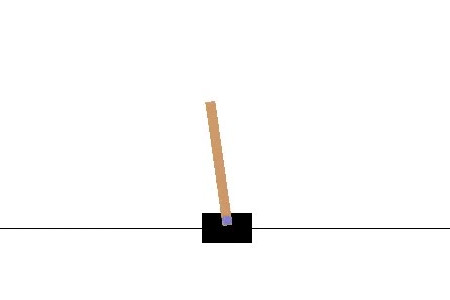
\includegraphics[width=7cm]{cartpole.jpg}
    \caption{The cartpole to balance verticaly. The cartpole can be seen as an inverted pendulum
    sitting on a small moving cart.}
\end{figure}

\begin{enumerate}
    \item Could we tackle this problem without machine learning ? Do you have any idea how ?
    \item Given the state vector of the cart pole, let us keep only 2 features, the angle of the
        pole and the cart velocity. How can you transform those continuous variables to
        categorical ones ? Why do you need to do so ?
    \item What is the reward function of this problem ? What are the possible actions ?
    \item Using Q Learning to solve this problem, what will be the dimensionnality of the Q table.
    \item What is the Bellman equation ? Where is it used in Q learning ?
    \item Using the provided template, implement you solution in python. 

\end{enumerate}

\reponse{
    (a) It could be done using regular control theory (\url{https://en.wikipedia.org/wiki/Inverted_pendulum)}\\

    (b) Create bins of values, since Q learning uses a Qtable we need to be able to categorize so that
    the number of cases in the table in finite. \\

    (c) +1 for each timestep it still balanced \\

    (d) If we keep only 2 features and categorize in 20 bins, and knowing that there are 2 possibles
    actions, the table will be : 20x20x2

    (e) The bellman equation is used to update the Q table at each timestep

    (f) see github for implementation
}

\end{Q}

\noindent
\rule{\textwidth}{0.4pt}
\footnotesize{Found an error? Let us know: \url{https://github.com/iridia-ulb/INFOH410/issues}}

\end{document} 
